\begin{figure}[h]
\centering
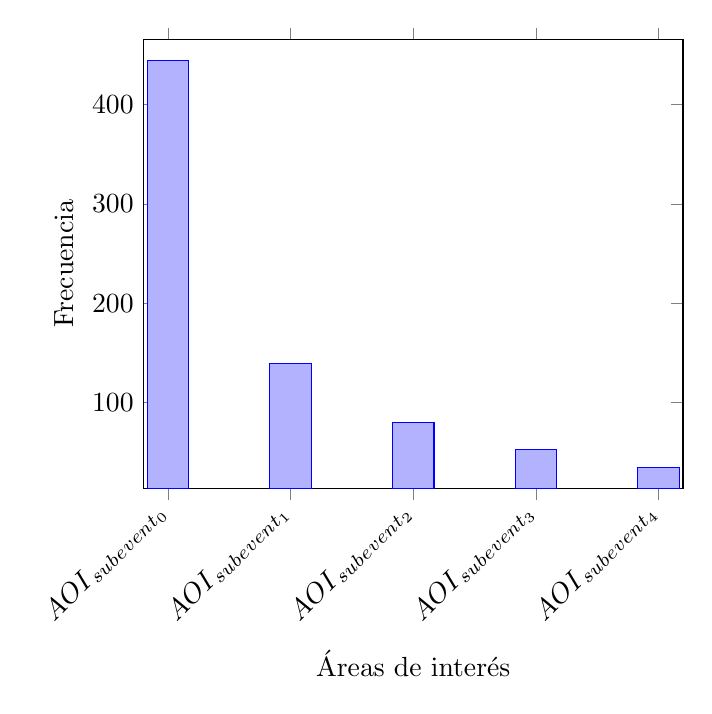
\begin{tikzpicture}
\begin{axis}[
    x tick label style={rotate=45, anchor=east},
    ylabel=Frecuencia,
    xlabel=Áreas de interés,
    enlargelimits=0.05,
    legend style={at={(0.5,-0.1)}, anchor=north,legend columns=-1},
    ybar,
    bar width=15pt,
    symbolic x coords={$\text{AOI}_{subevent_0}$,$\text{AOI}_{subevent_1}$,$\text{AOI}_{subevent_2}$,$\text{AOI}_{subevent_3}$,$\text{AOI}_{subevent_4}$},
    xtick=data
]
\addplot coordinates {
    ($\text{AOI}_{subevent_0}$, 445)
    ($\text{AOI}_{subevent_1}$, 139)
    ($\text{AOI}_{subevent_2}$, 80)
    ($\text{AOI}_{subevent_3}$, 52)
    ($\text{AOI}_{subevent_4}$, 34)
};
\end{axis}
\end{tikzpicture}
\end{figure}